\documentclass[11pt]{article}
\usepackage{polyglossia}
\usepackage{graphicx}
\usepackage{caption}
\usepackage{subcaption}
\setmainlanguage{french}
\PolyglossiaSetup{french}{indentfirst=true}
\usepackage{longtable}
\usepackage{enumerate}
\usepackage{tabularx}
\usepackage[french,onelanguage]{algorithm2e}
\usepackage{incgraph,tikz}
\usepackage{geometry}
\usepackage{amsmath}
\geometry{top=3cm, bottom=3cm, left=3cm, right=3cm}
\usepackage{float}
\usepackage{pdfpages}

\usepackage{listings}
\lstset{
basicstyle=\small\ttfamily,
columns=flexible,
breaklines=true
}

\newenvironment{myitemize}
{ \begin{itemize}
    \setlength{\itemsep}{0pt}
    \setlength{\parskip}{0pt}
    \setlength{\parsep}{0pt}     }
{ \end{itemize}                  } 

\usepackage{tikz}
\def\checkmark{\tikz\fill[scale=0.4](0,.35) -- (.25,0) -- (1,.7) -- (.25,.15) -- cycle;}

\usepackage{titlesec}

\setcounter{secnumdepth}{4}

\titleformat{\paragraph}
{\normalfont\normalsize\bfseries}{\theparagraph}{1em}{}
\titlespacing*{\paragraph}
{0pt}{3.25ex plus 1ex minus .2ex}{1.5ex plus .2ex}




\title{TP Programmation Concurrente}
\author{Groupe B3425 ({\sc Espeute} Clément, {\sc Gao} Yiqin)}
\makeatletter

\begin{document}
\maketitle

\section{Changements apportés par rapport à la conception initiale}

\begin{itemize}
	\item Nous avons ajouté une boite aux lettres entre les Tâches Clavier et Sortie, affin que Clavier puisse communiquer à Sortie les voitures qui doivent quitter le parking.
	\item Nous avons aussi ajouté la tâche heure qui avait était oubliée à la conception initiale.
	
	\item Nous avons remplacé l’utilisation de SIGUSR1 par un sémaphore entre Sortie et Entree pour communiquer qu'il faut faire rentrer une voiture suite à la libération d'une place dans le parking.
	
	\item Les deux mémoires partagées ont été fusionnées en une seule, dans une structure VoituresParking qui contient à présent le nombre de places libres dans le parking, les voitures qui y sont garées et les voitures qui attendent aux barrières.
\end{itemize}




\newpage
\incgraph[paper=current,options={width=18cm}]{MereInit.png}
\incgraph[paper=current,options={width=18cm}]{MereDestr.png}
\incgraph[paper=current,options={width=18cm}]{EntreeInit.png}
\incgraph[paper=current,options={width=18cm}]{EntreeMoteur.png}
\incgraph[paper=current,options={width=18cm}]{MoteurDestruction.png}
\incgraph[paper=current,options={width=18cm}]{EntreeHandler.png}

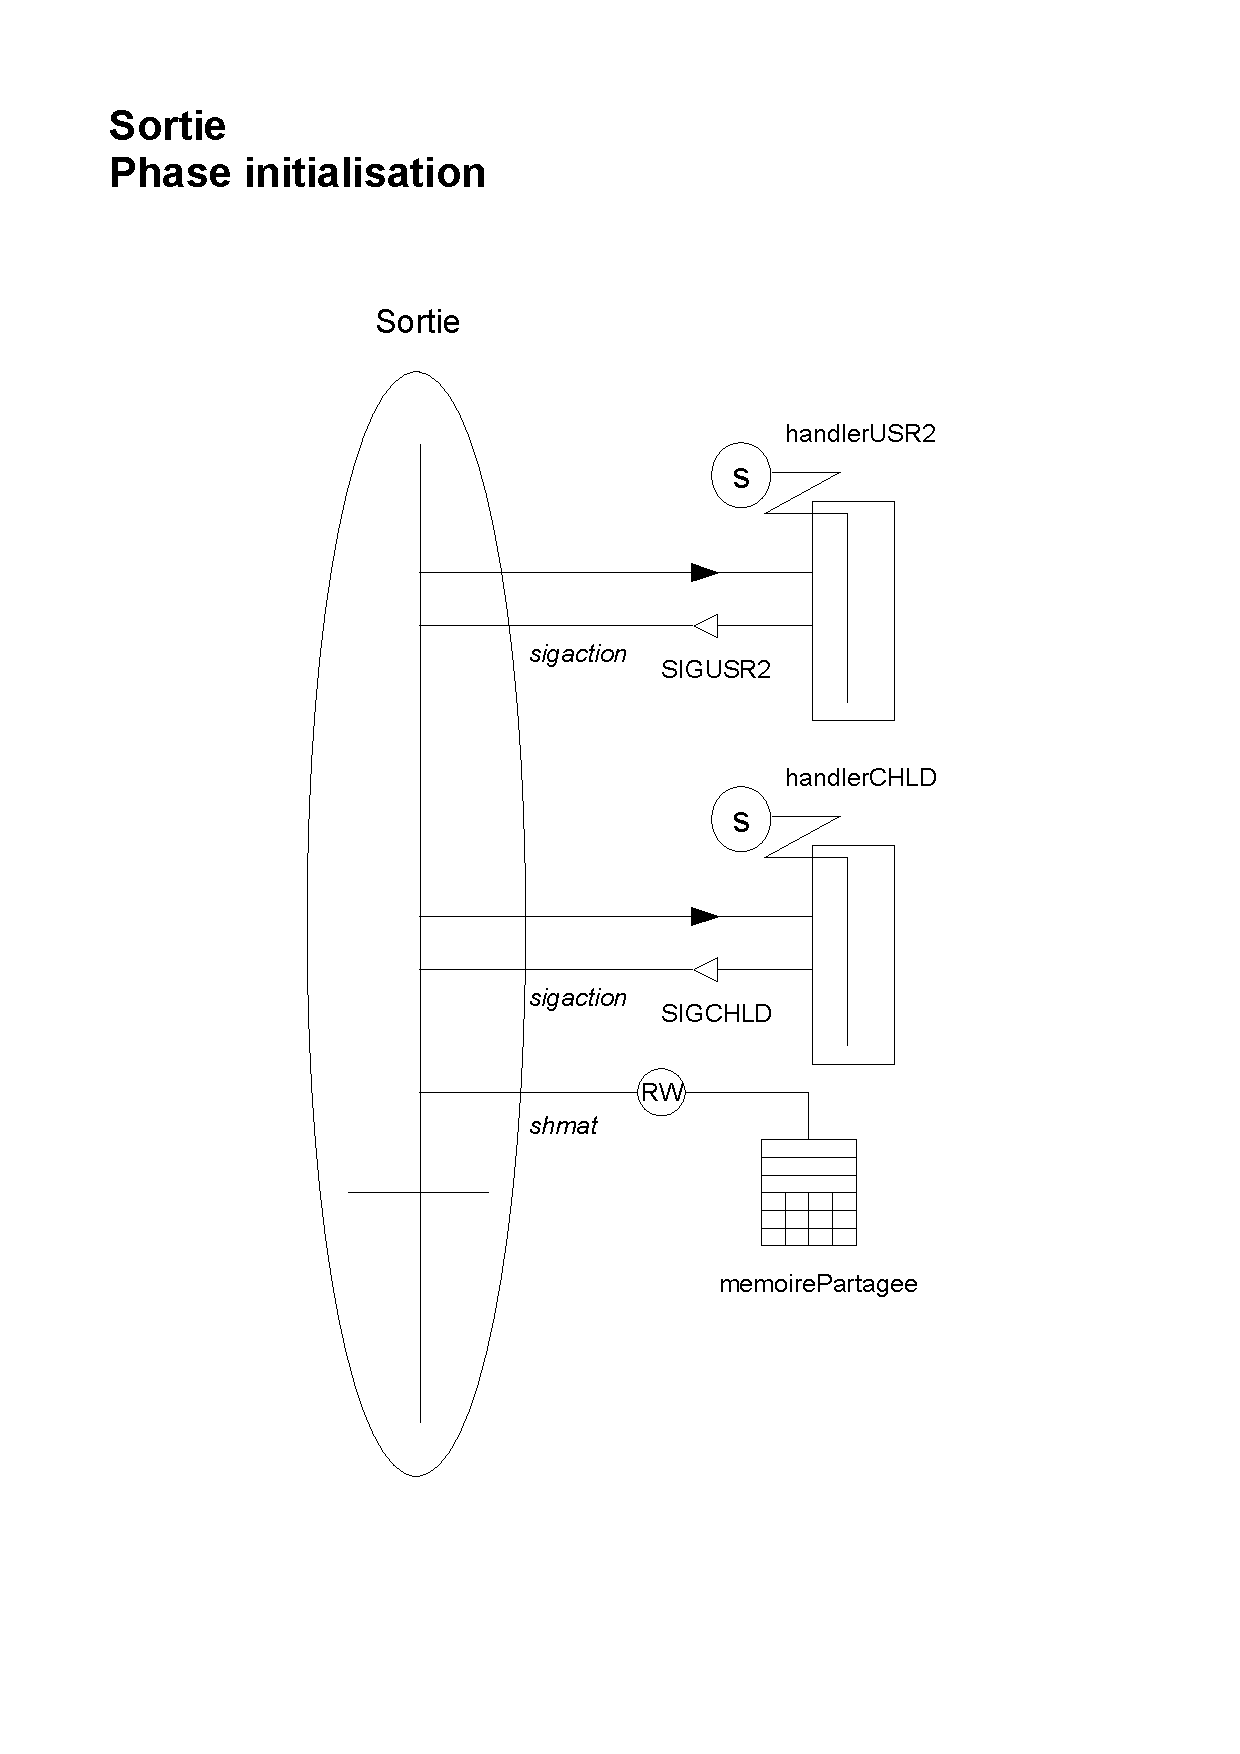
\includepdf[pages={-}]{Clavier-Sortie.pdf}

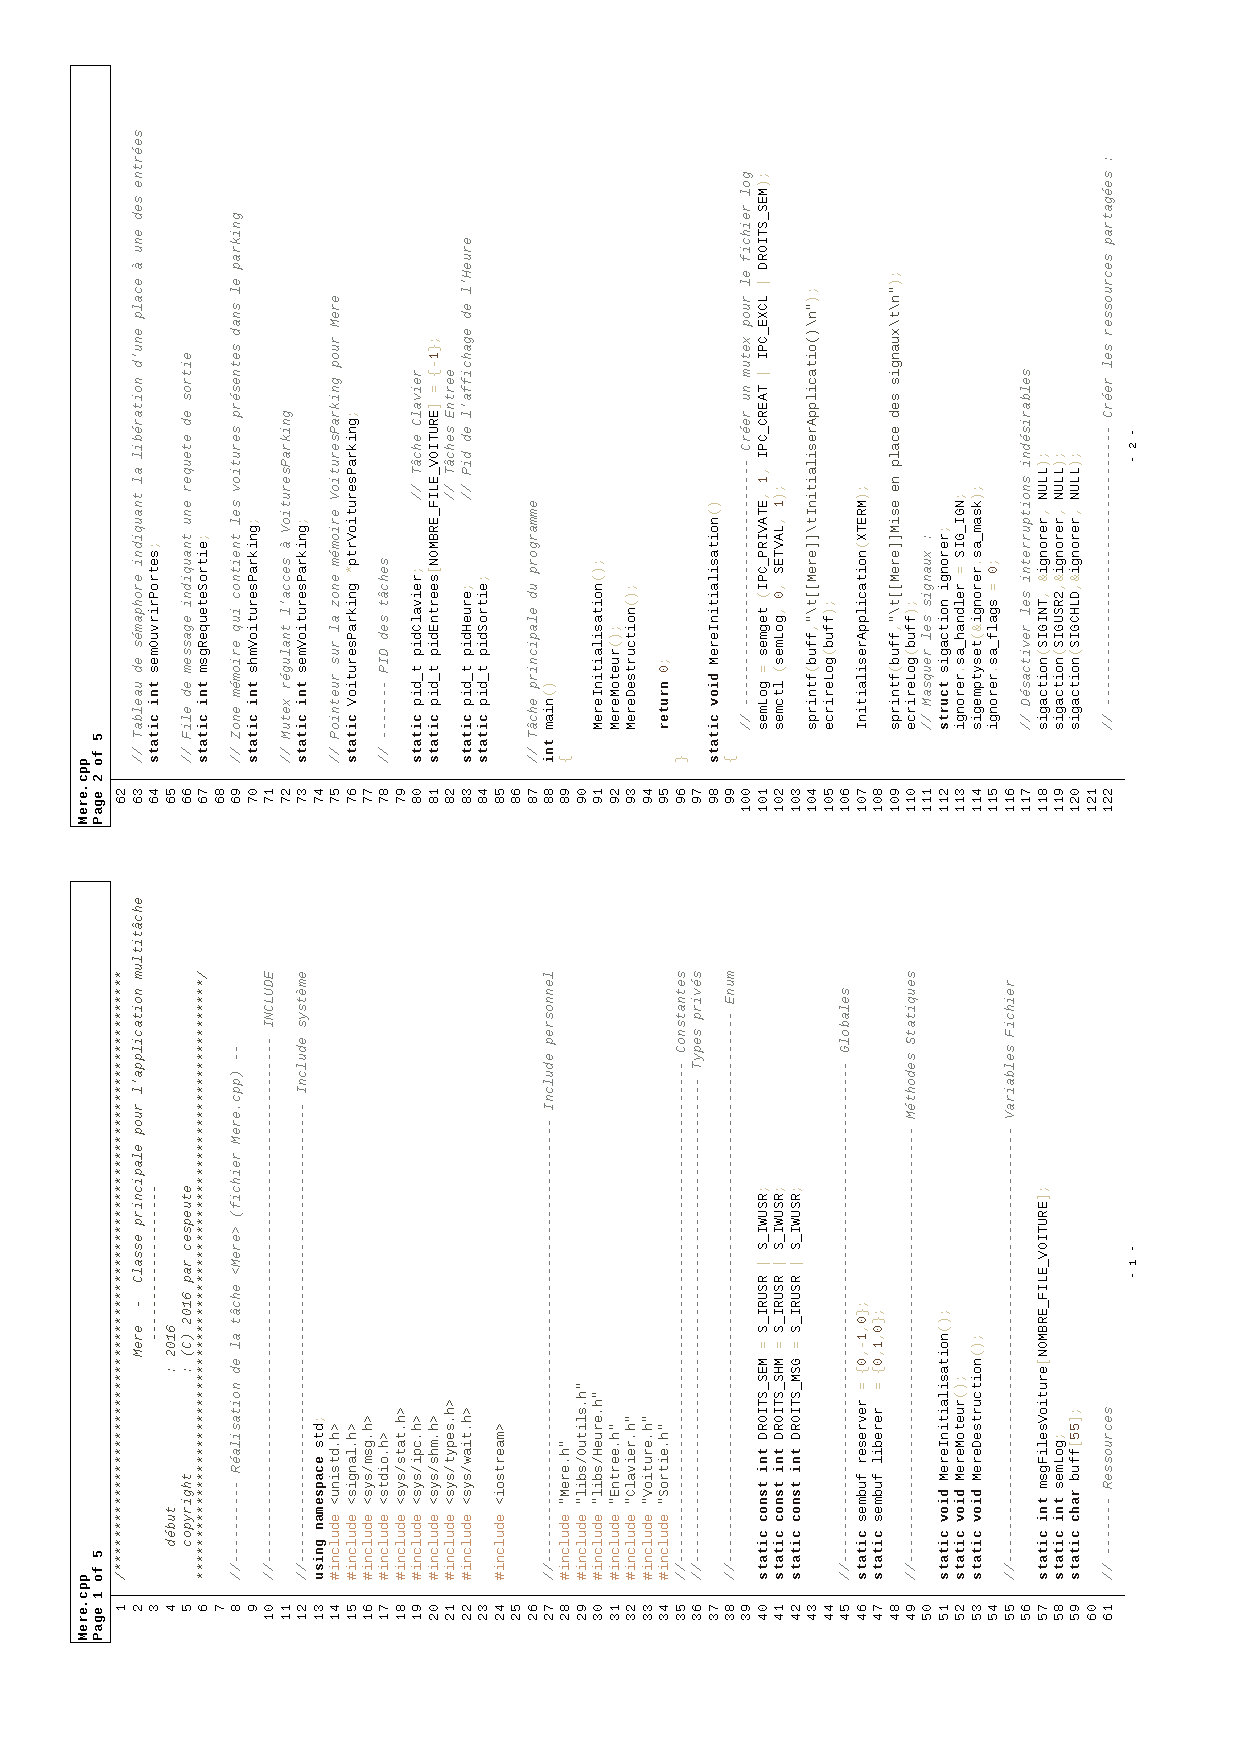
\includepdf[pages={-}]{Merecpp.pdf}
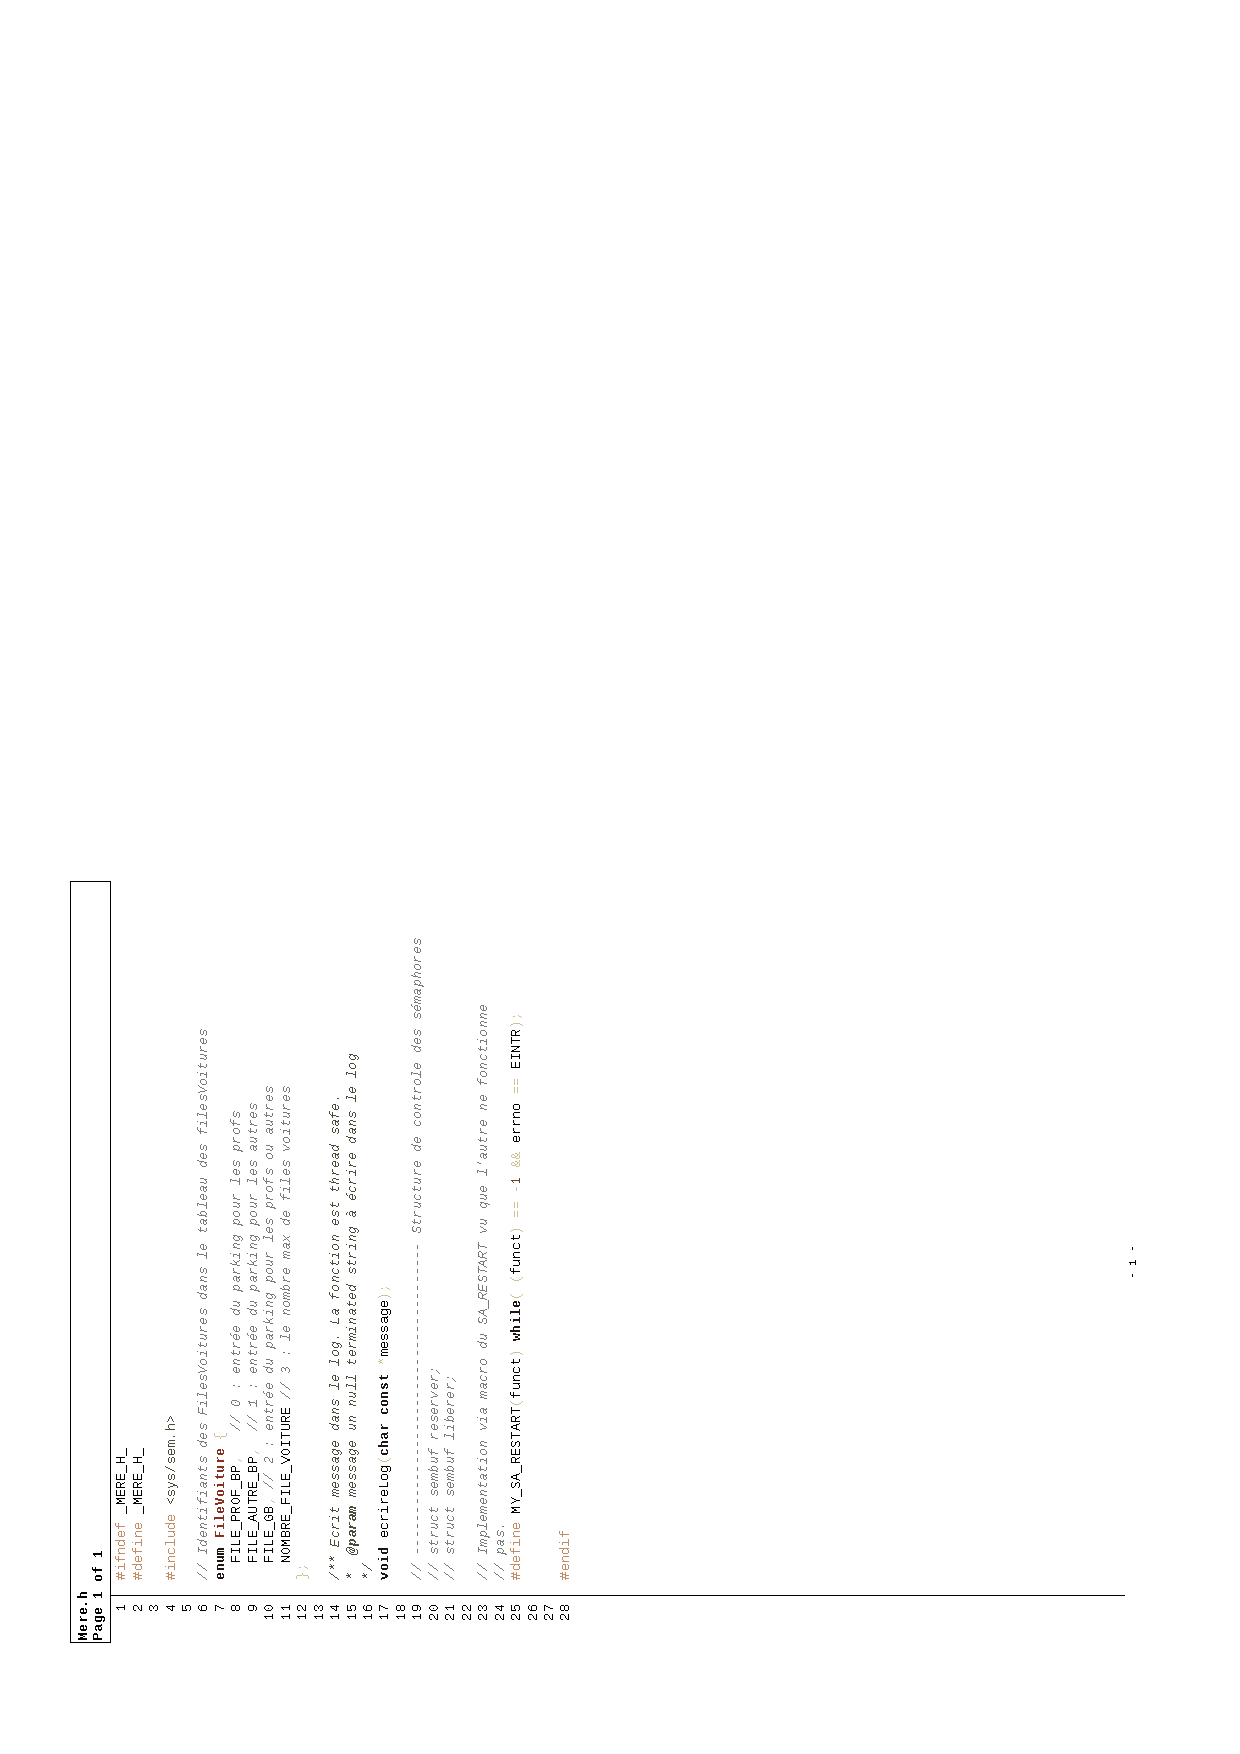
\includepdf[pages={-}]{Mereh.pdf}
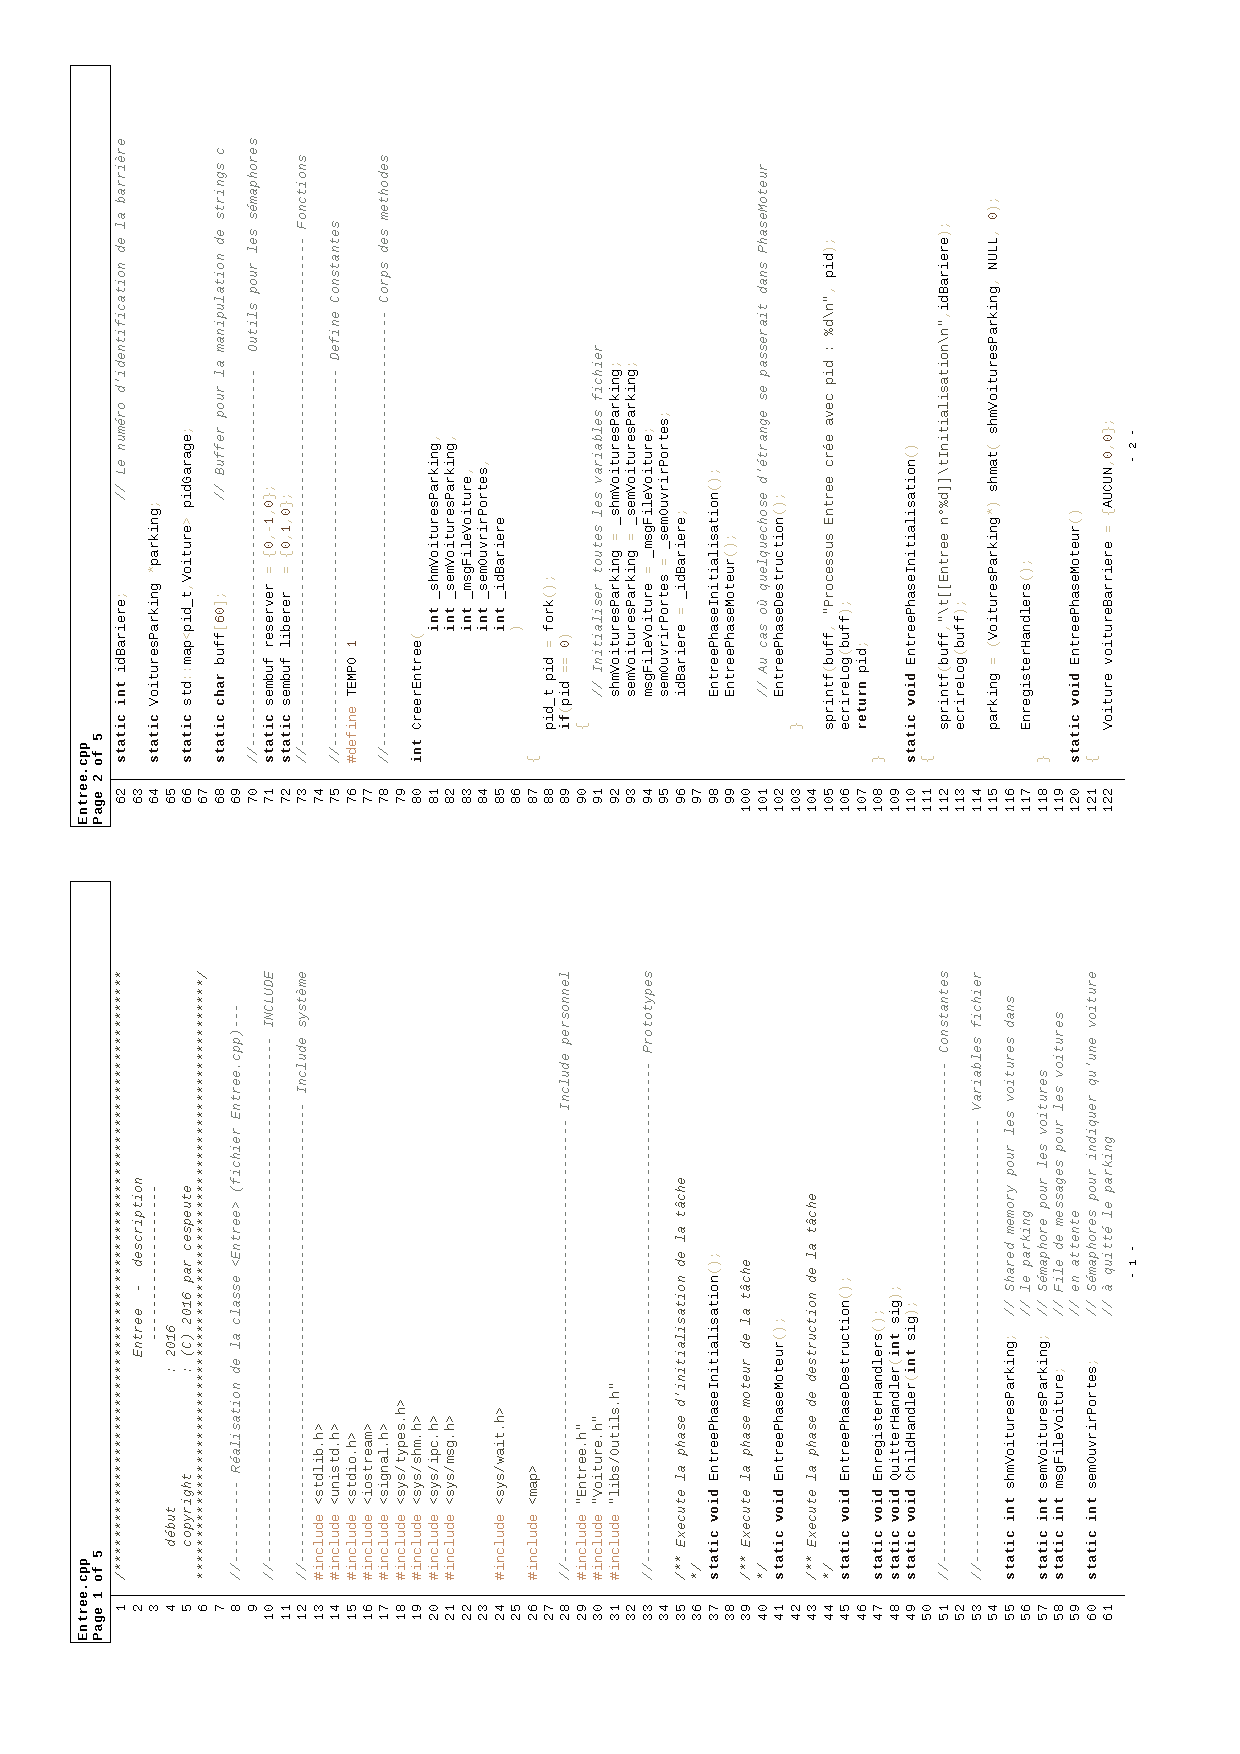
\includepdf[pages={-}]{Entreecpp.pdf}
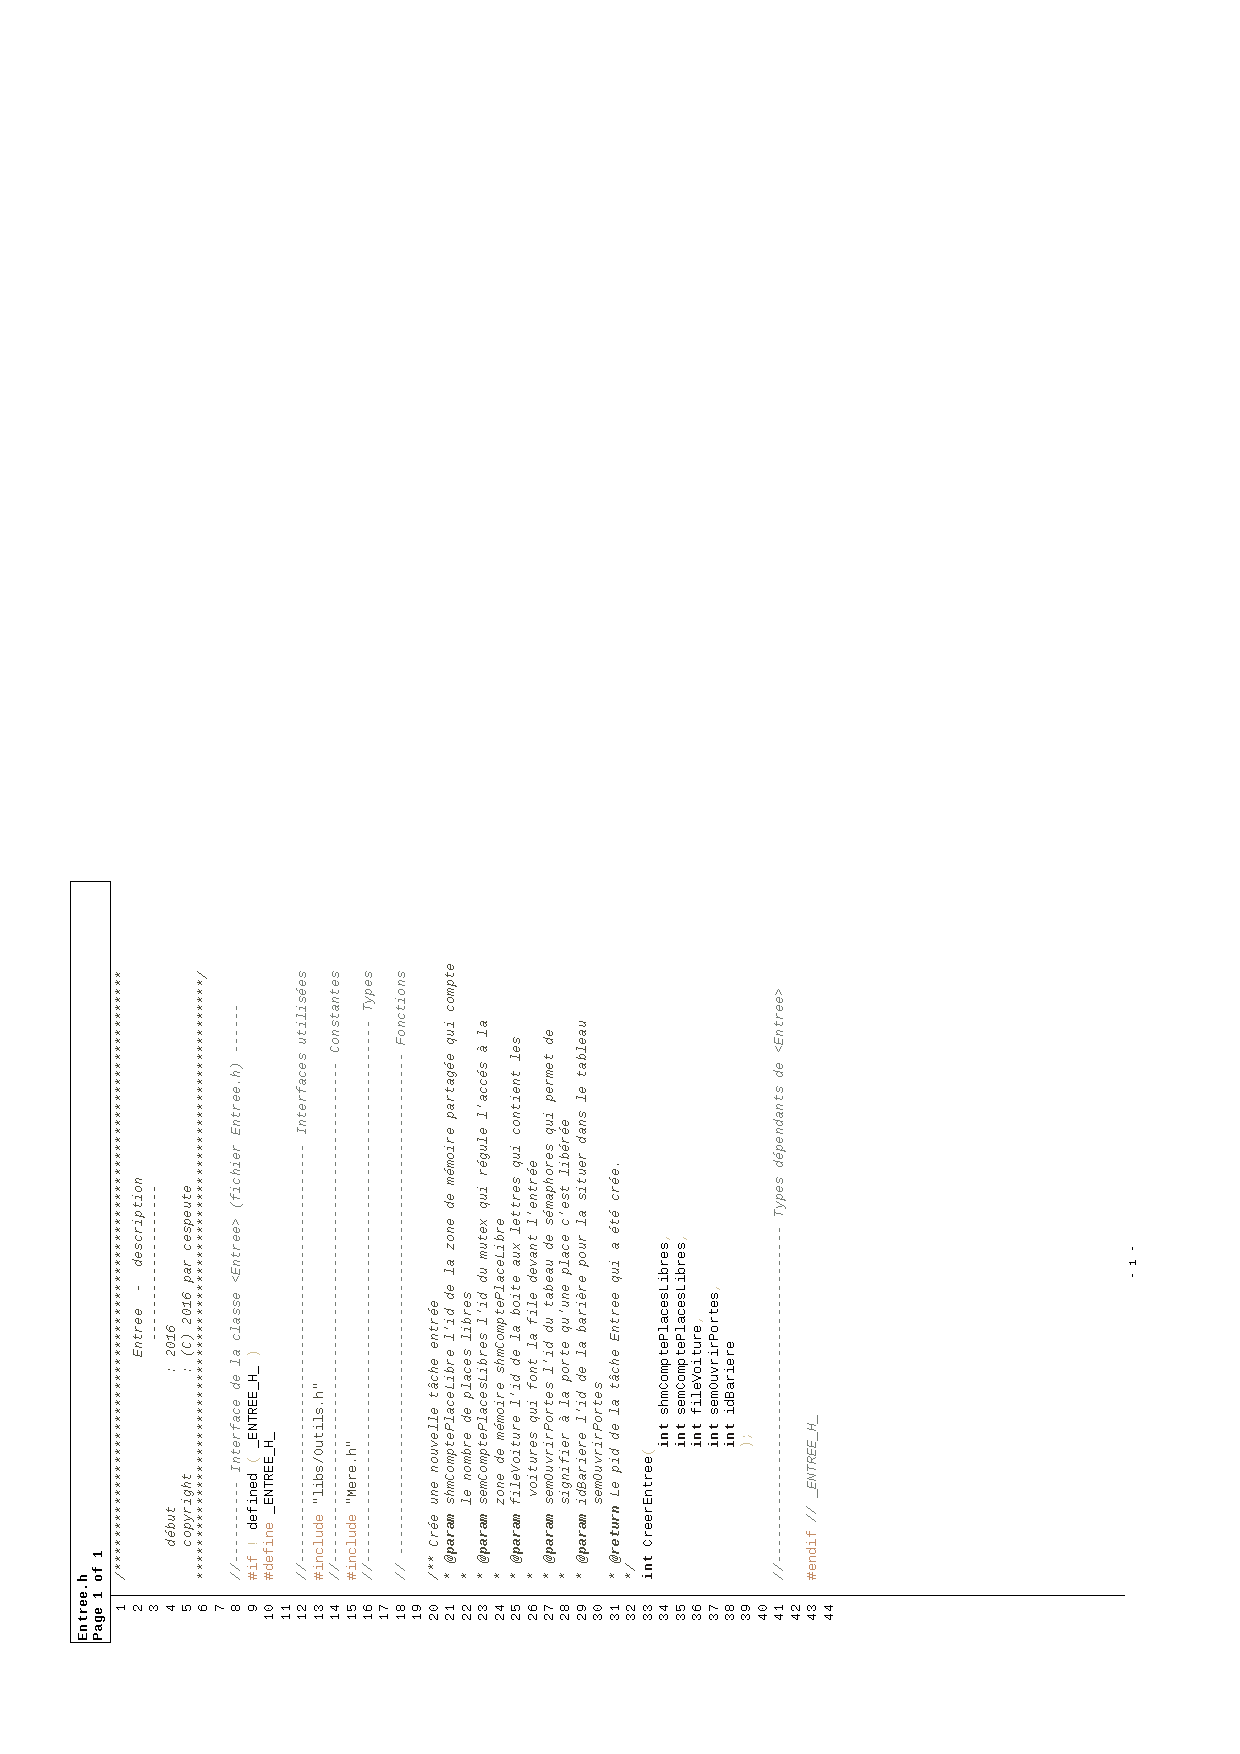
\includepdf[pages={-}]{Entreeh.pdf}
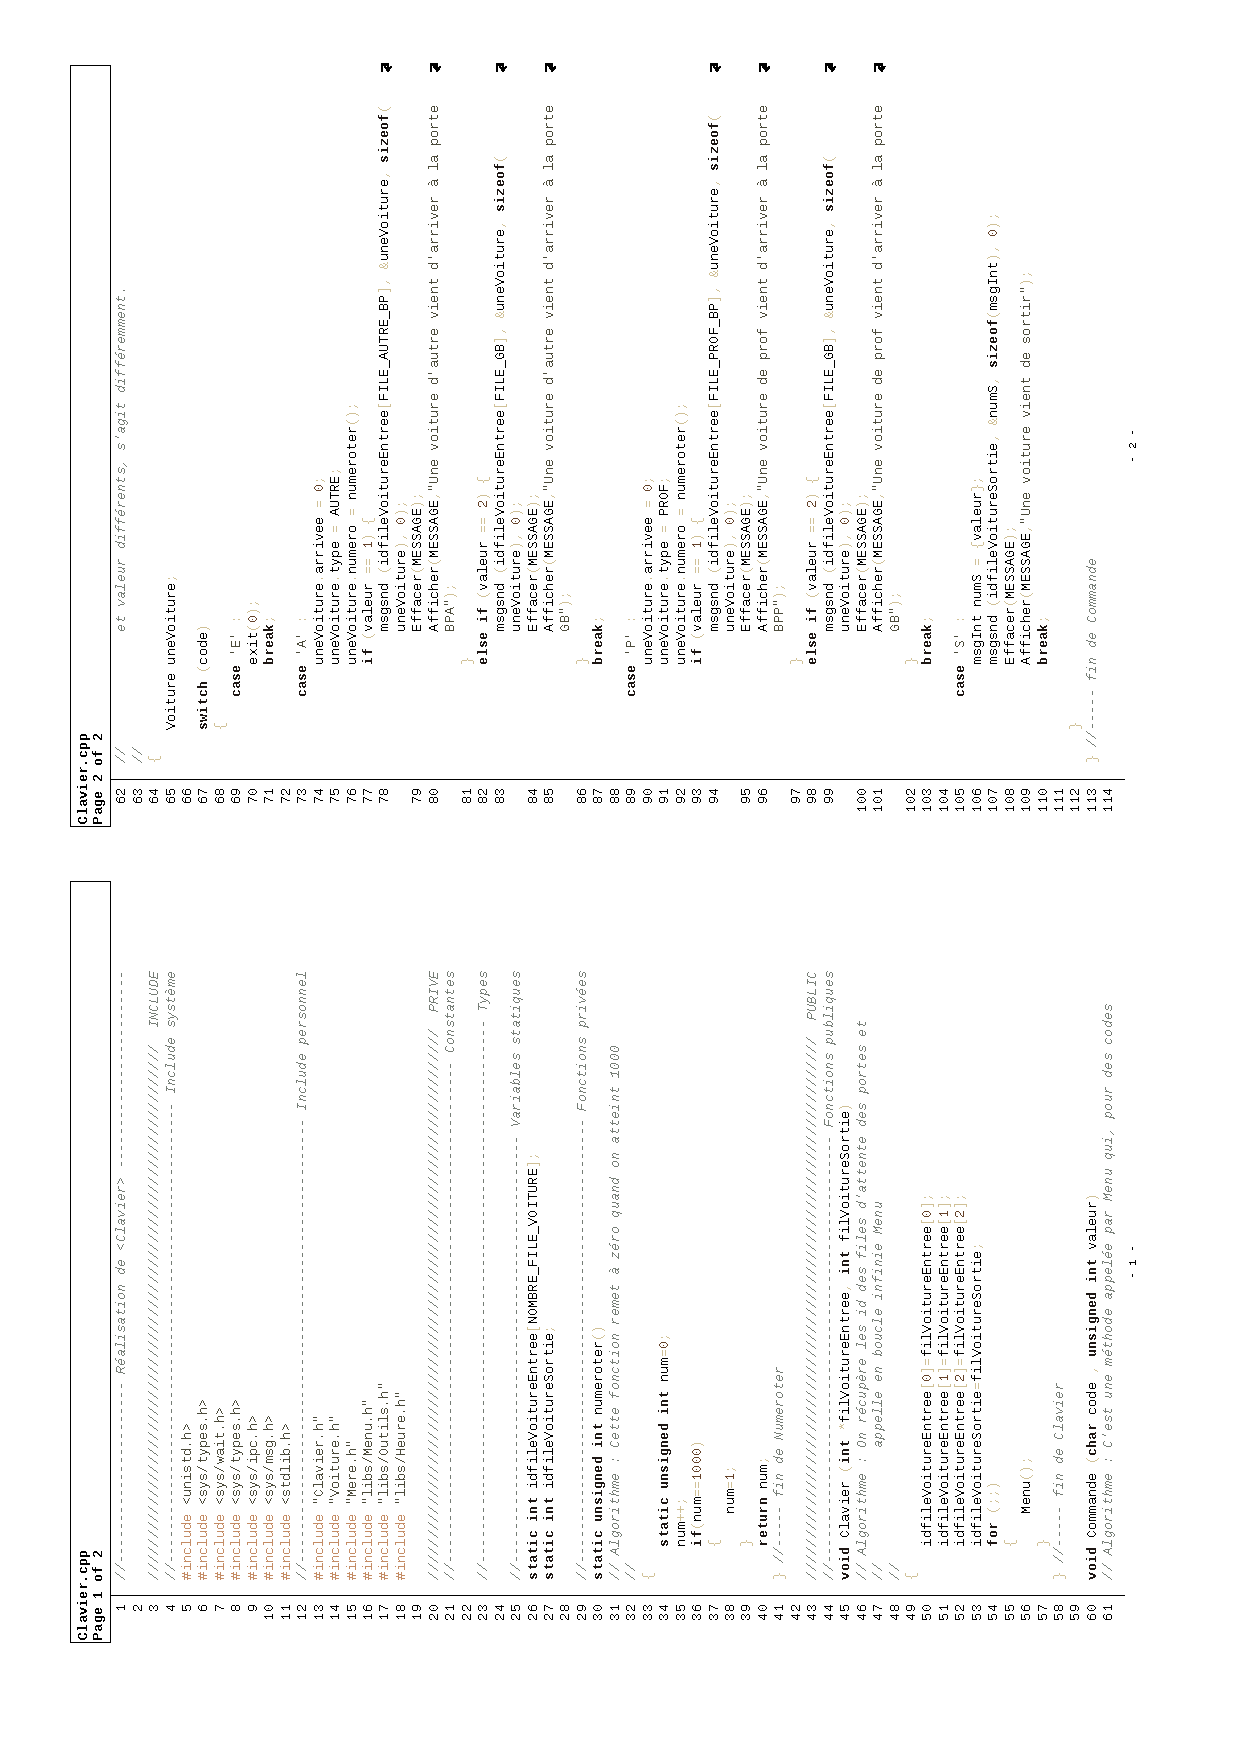
\includepdf[pages={-}]{Claviercpp.pdf}
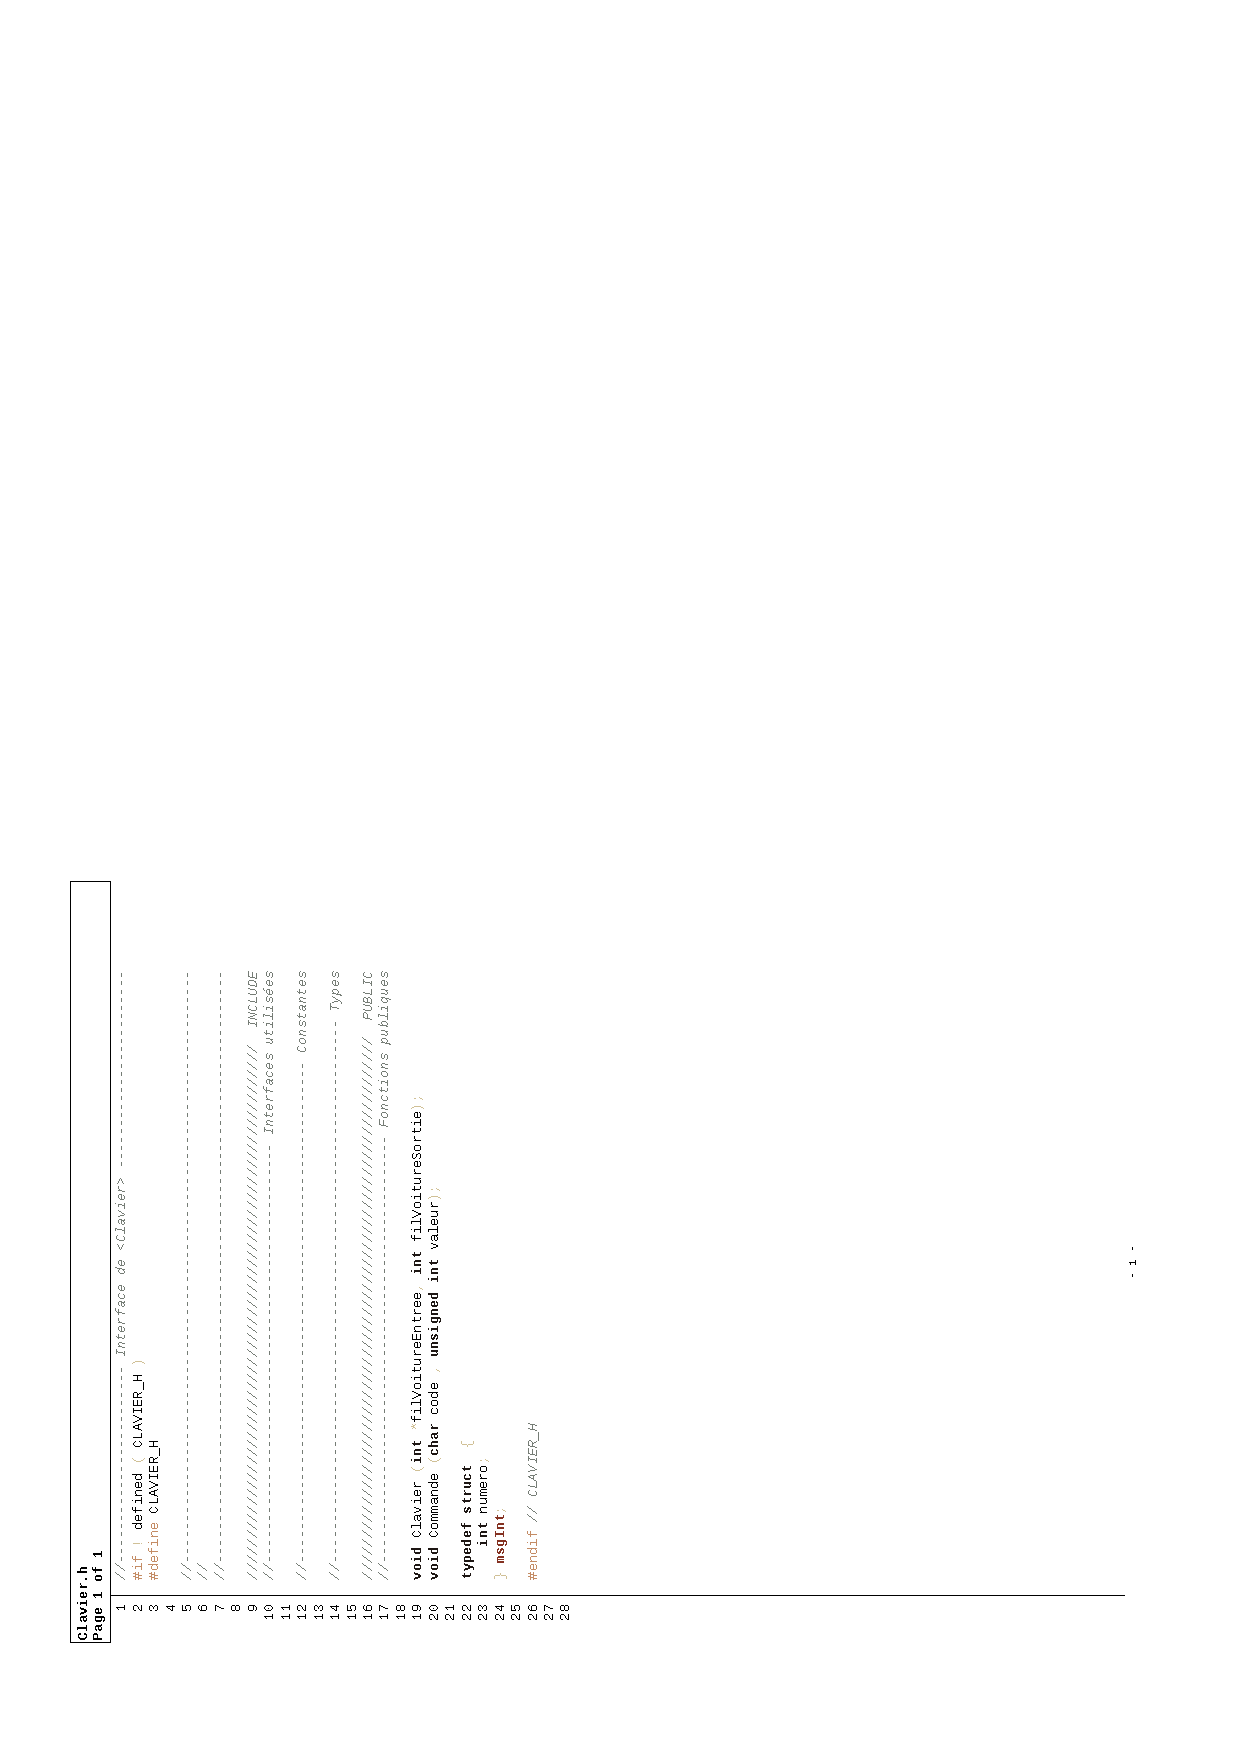
\includepdf[pages={-}]{Clavierh.pdf}
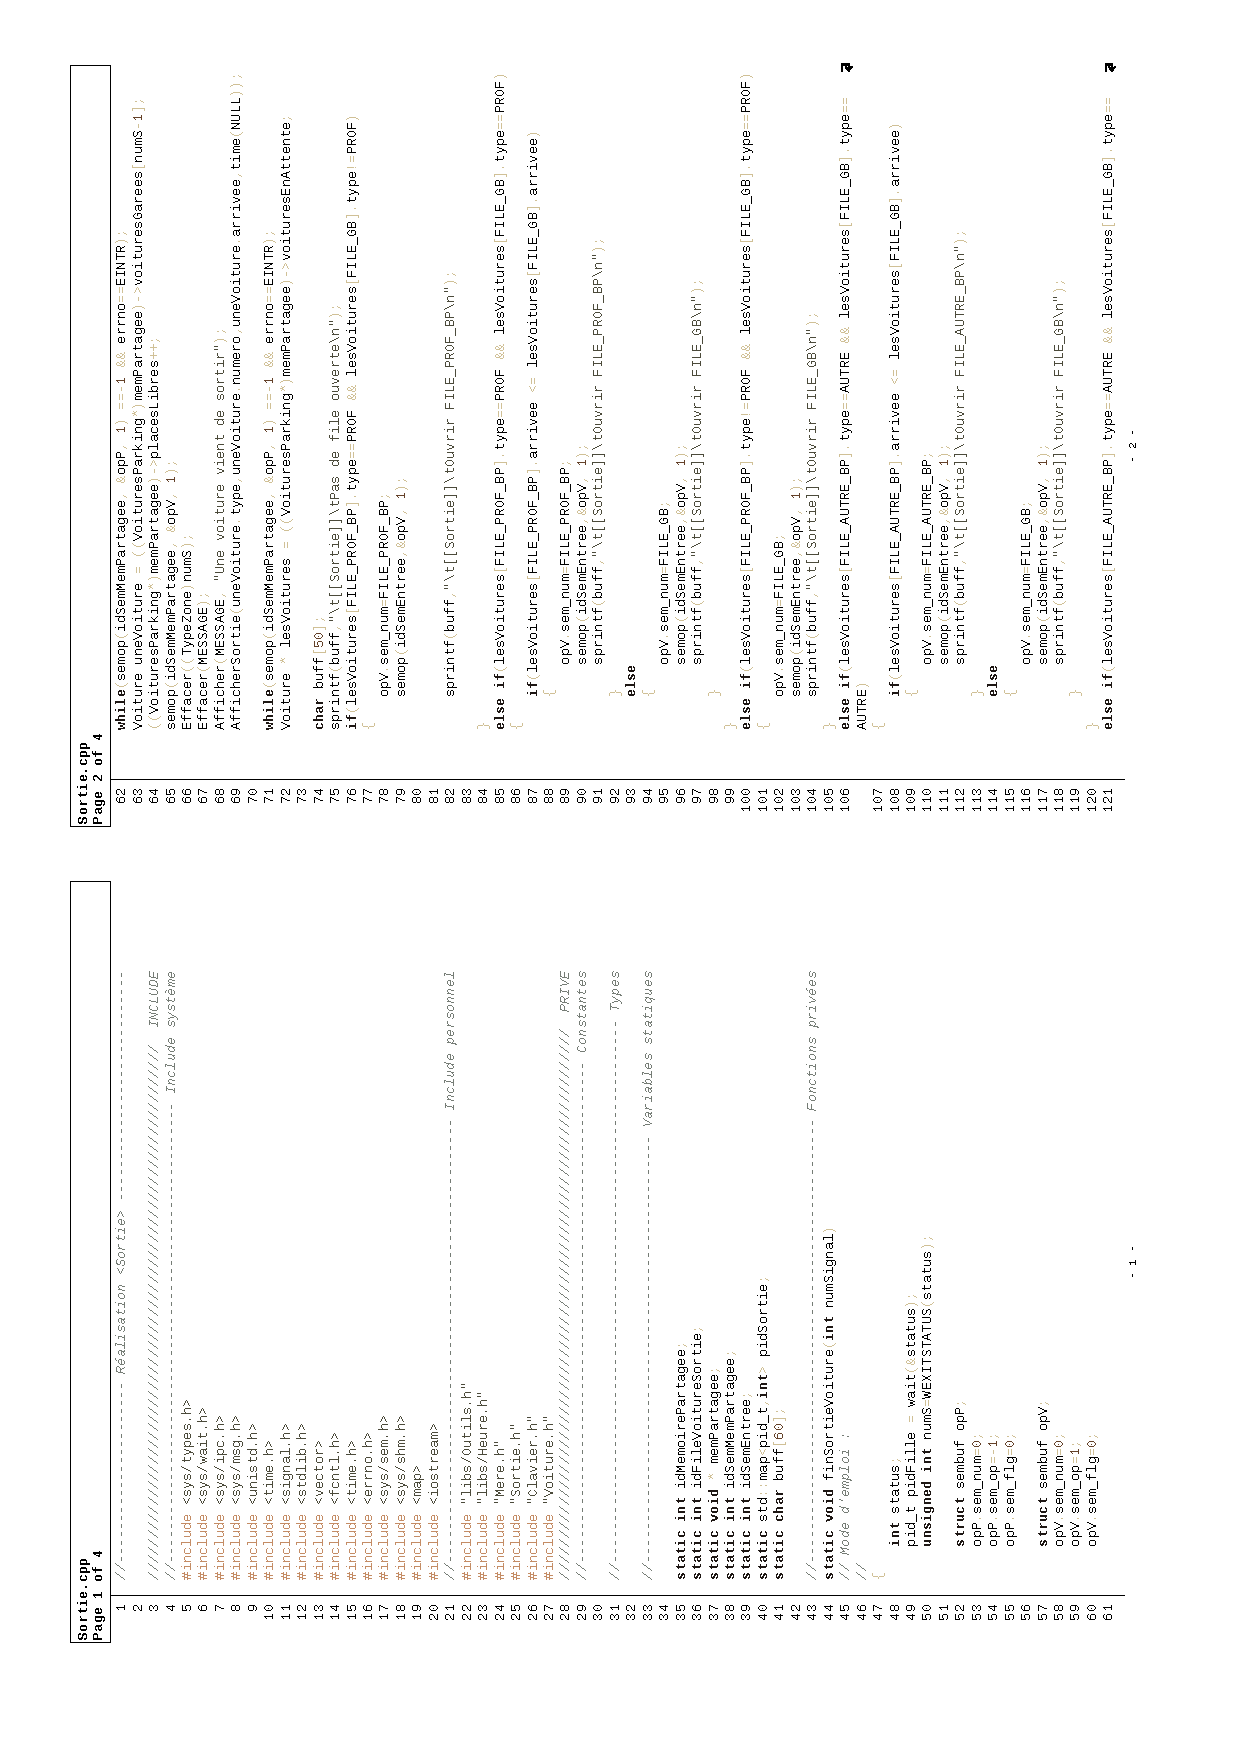
\includepdf[pages={-}]{Sortiecpp.pdf}
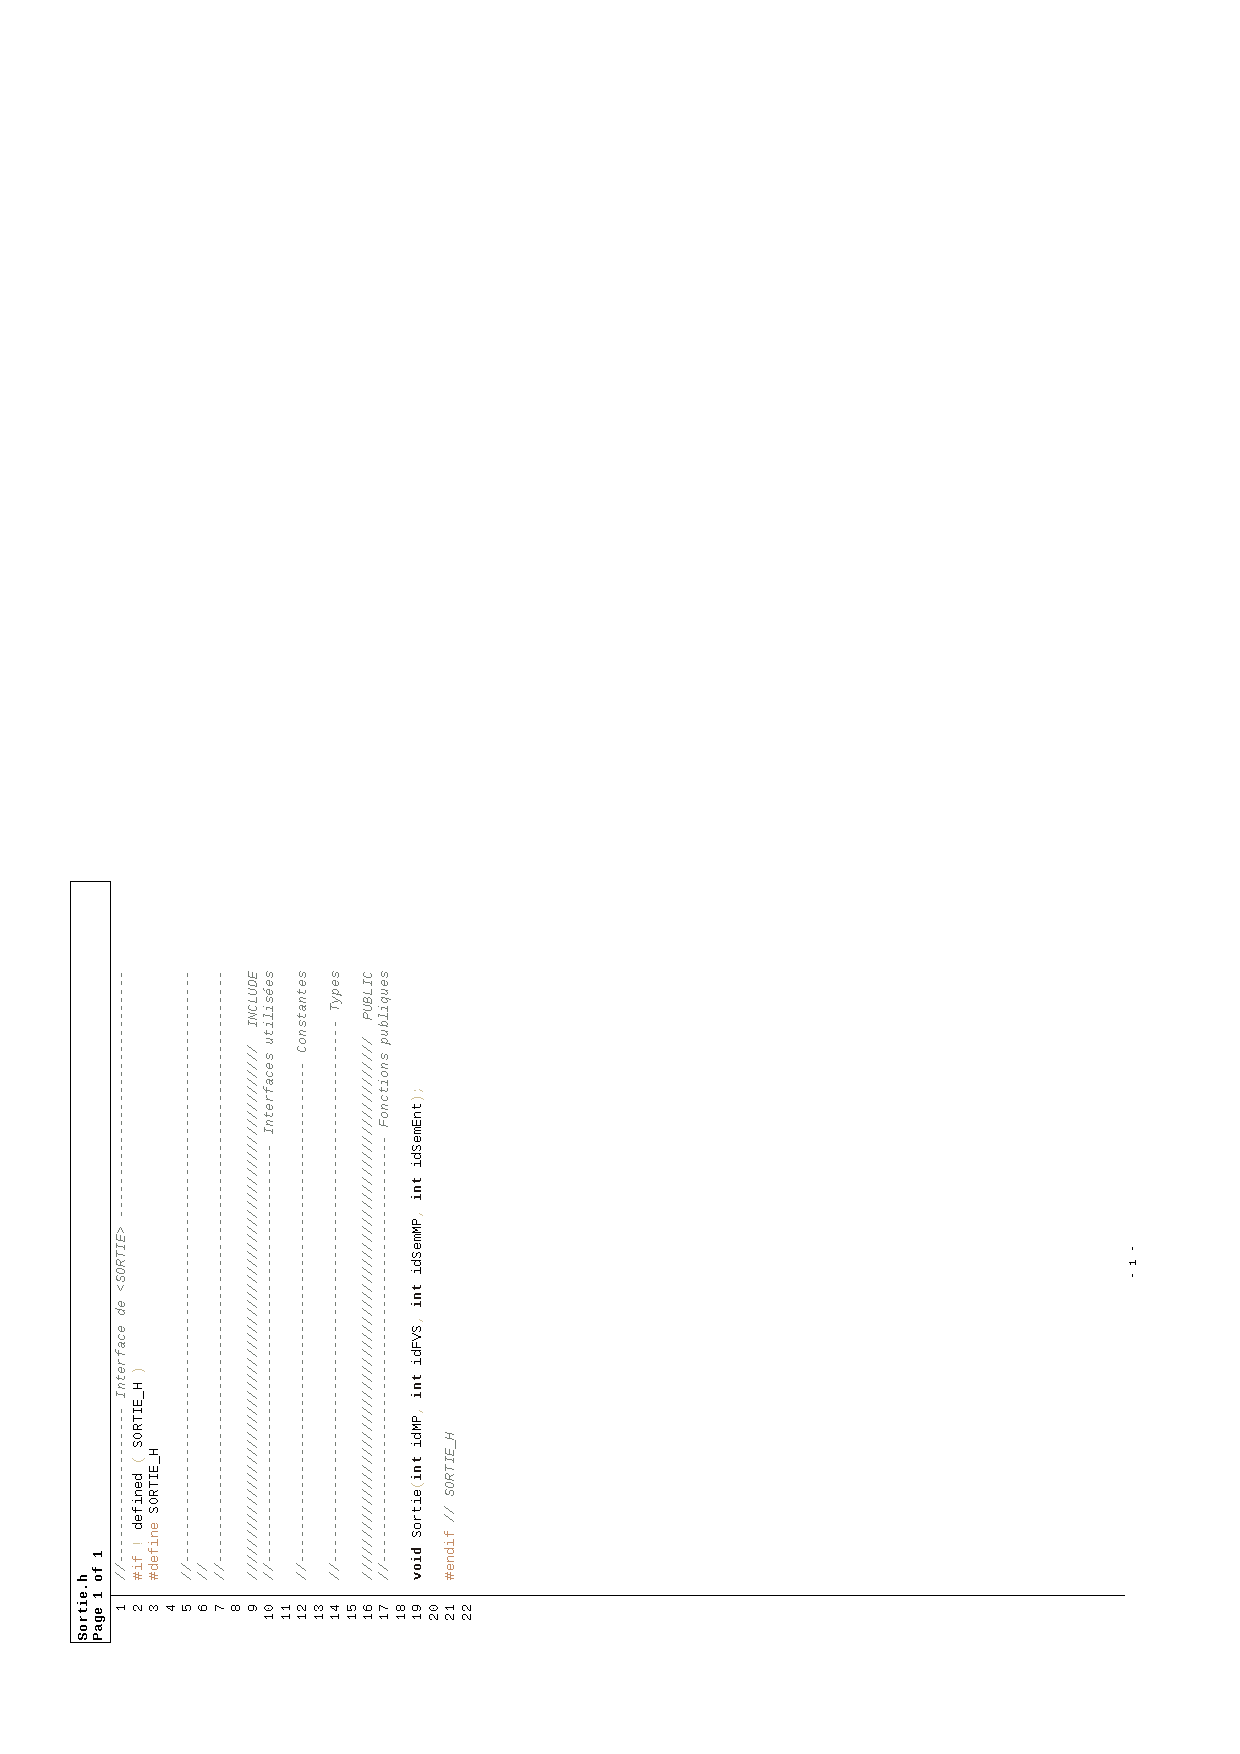
\includepdf[pages={-}]{Sortieh.pdf}

\end{document}